\section{Incarnation 1}
  \begin{flushleft}
    The logic for computing Cos, Sin, Pi and other functions were written from the ground up. See snippets below.
  \end{flushleft}
  \subsection{Snippets}
  \vspace{2em}
    \begin{figure}[h!]
      \centering
      \frame{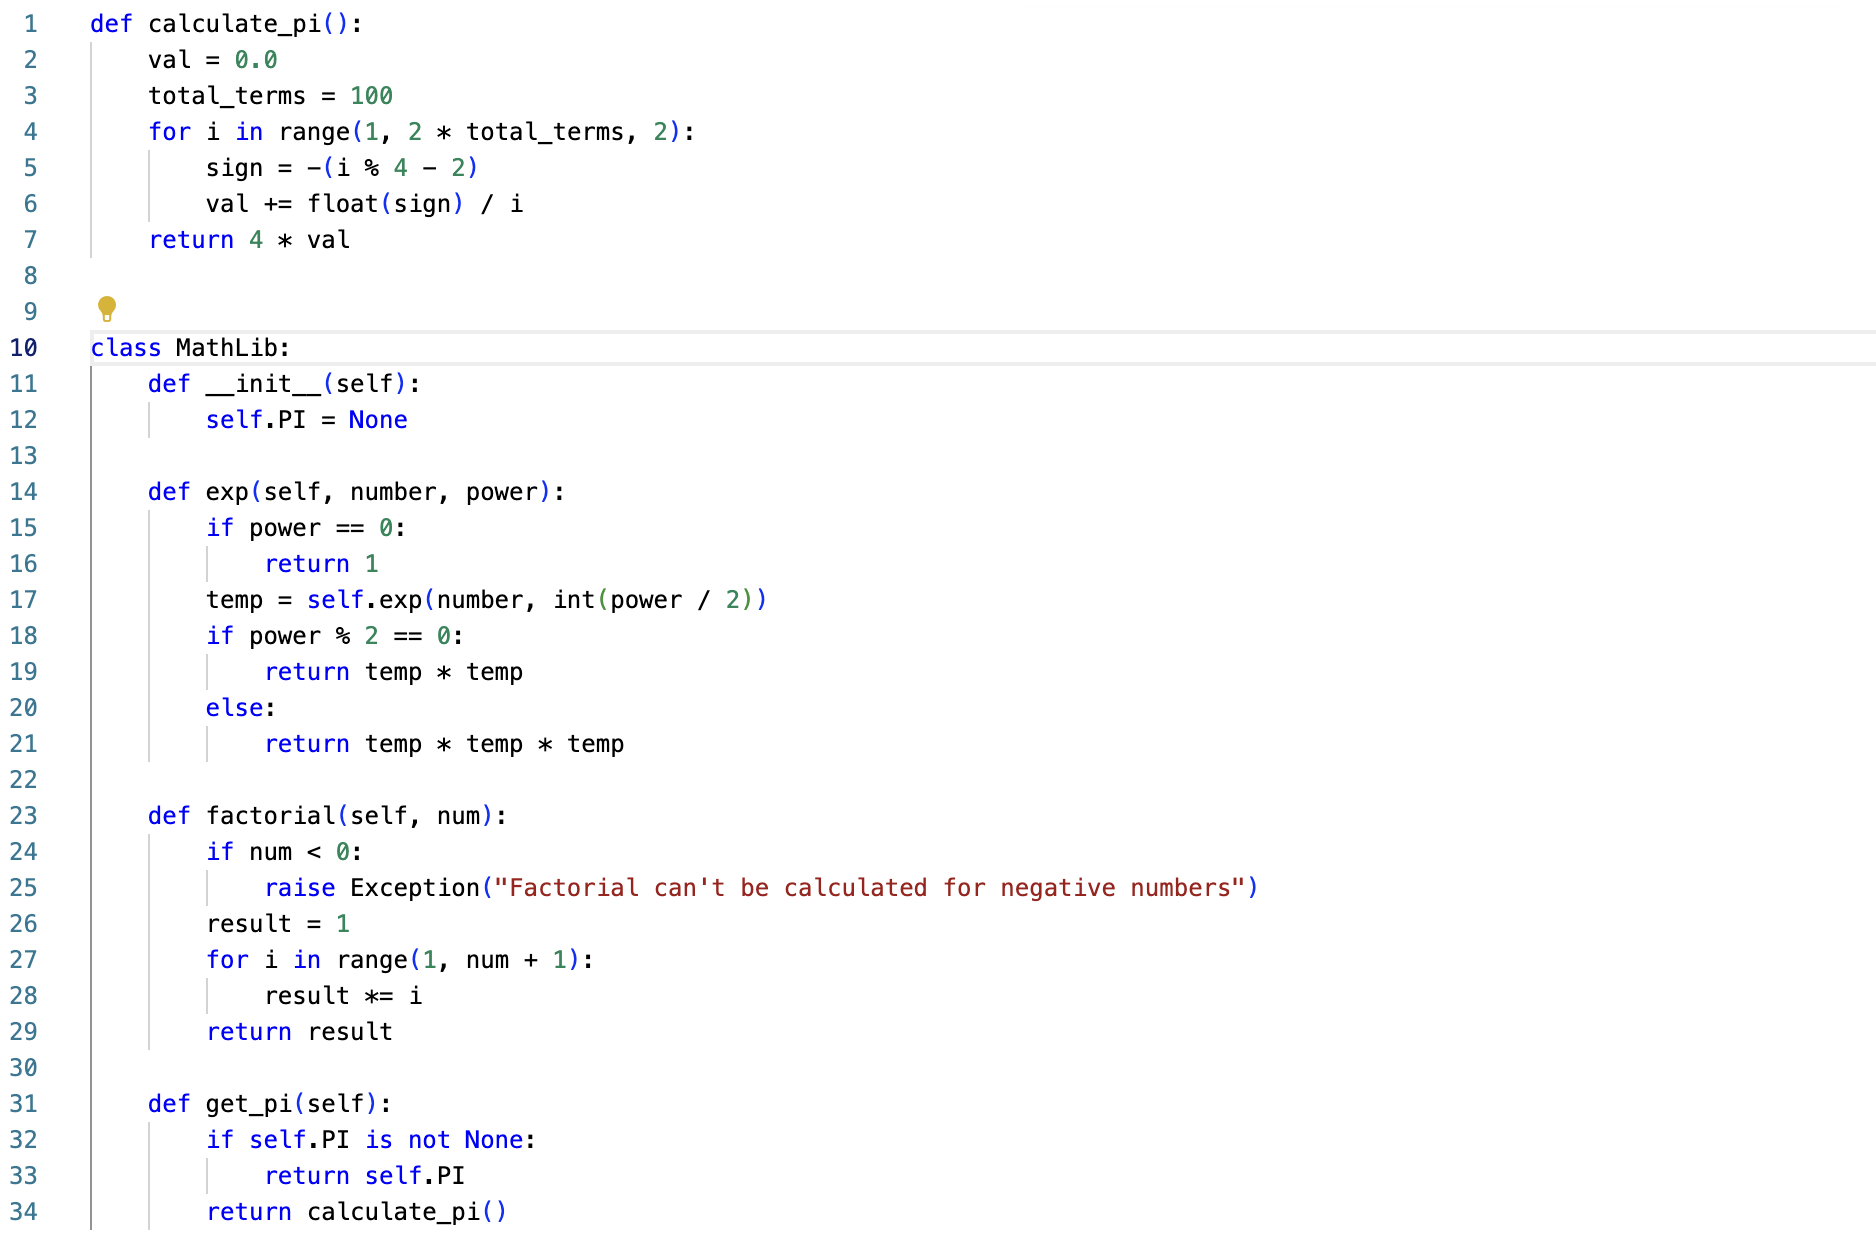
\includegraphics[scale= 0.4]{resources/snippets/Math.png}}
      \caption{Logic to compute Exponent, Factorial and Pi}
      \label{fig:Math Library}
    \end{figure}
    \pagebreak
    \begin{figure}[h!]
      \centering
      \frame{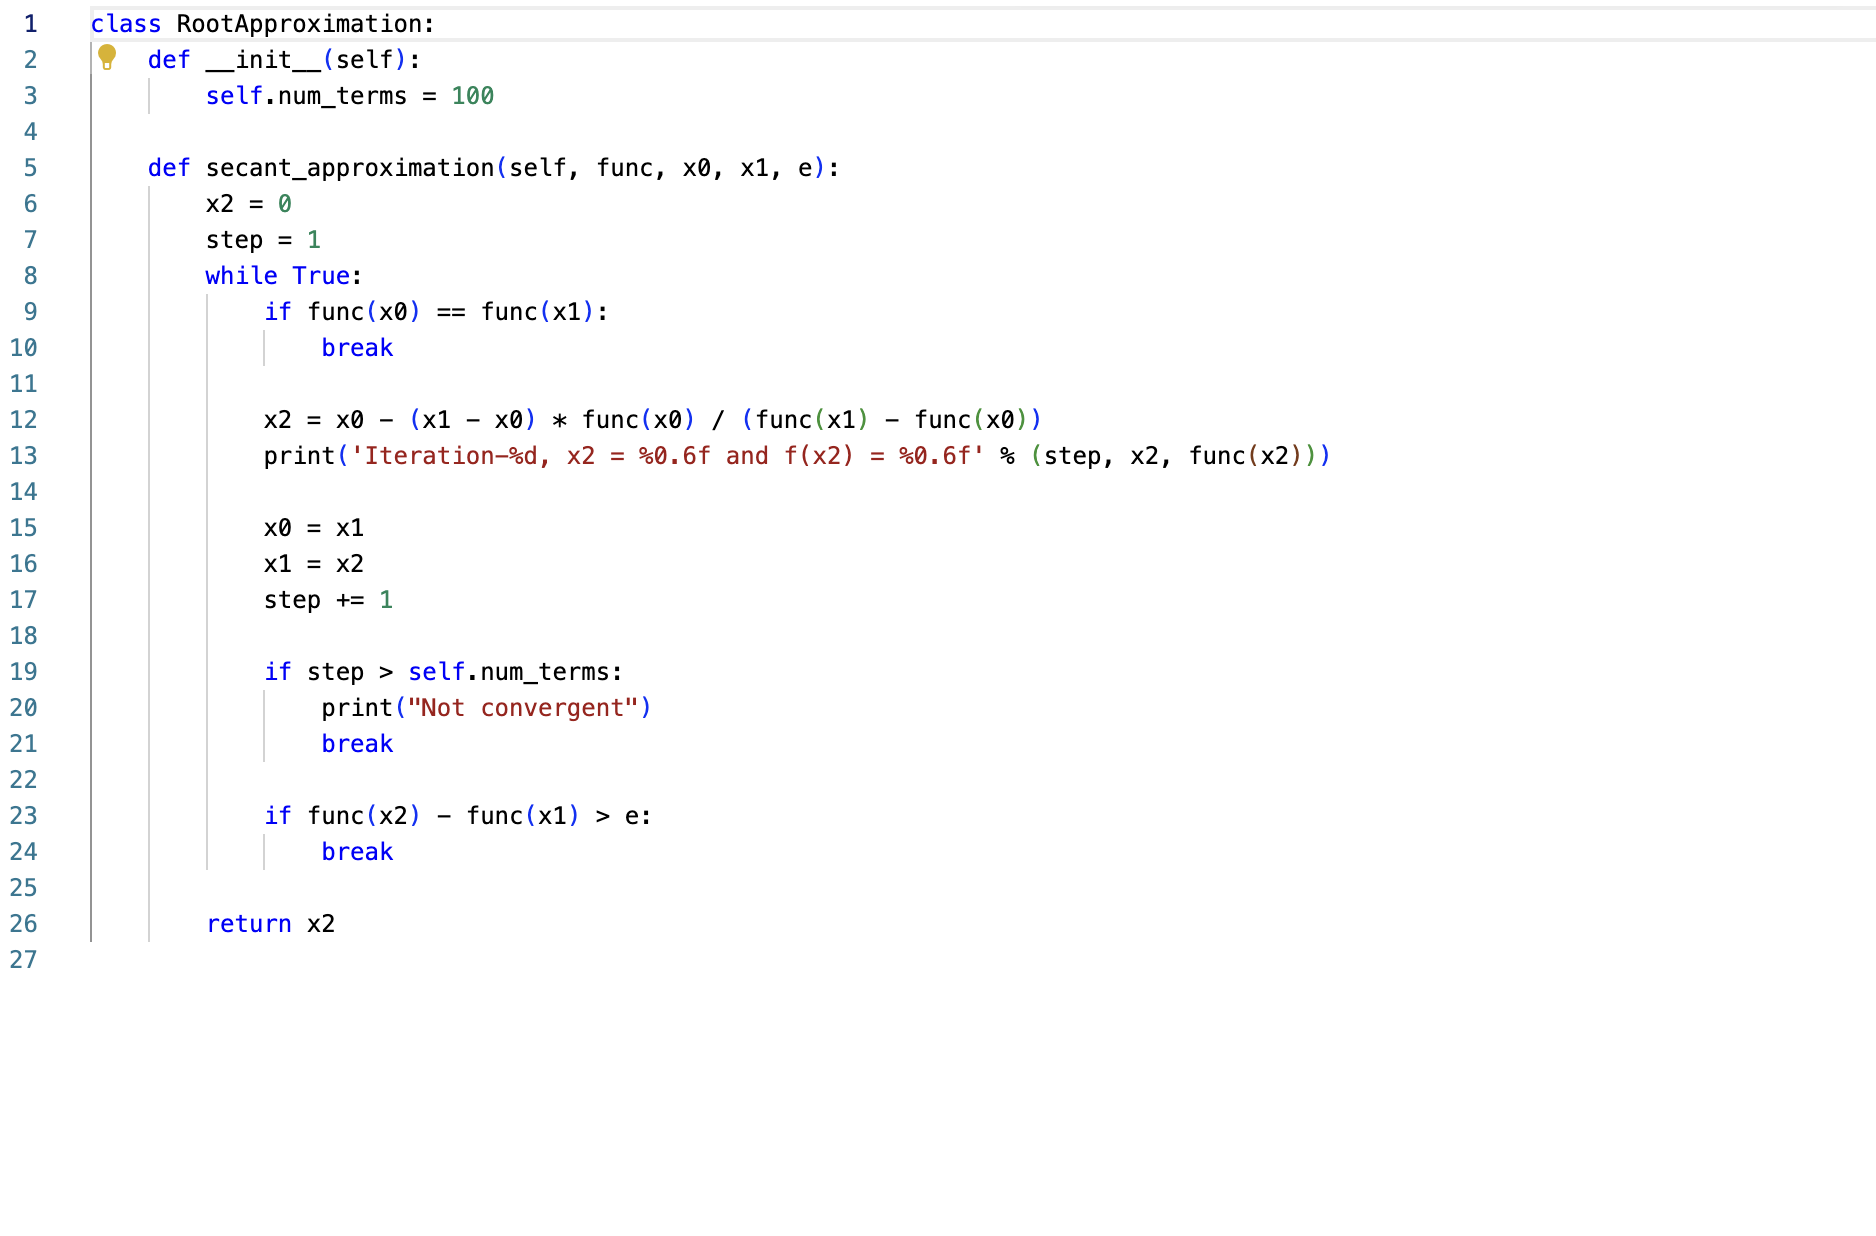
\includegraphics[scale= 0.4]{resources/snippets/Roots.png}}
      \caption{Secant Method of root approximation}
      \label{fig:Root Approximation}
    \end{figure}

    \begin{figure}[h!]
      \centering
      \frame{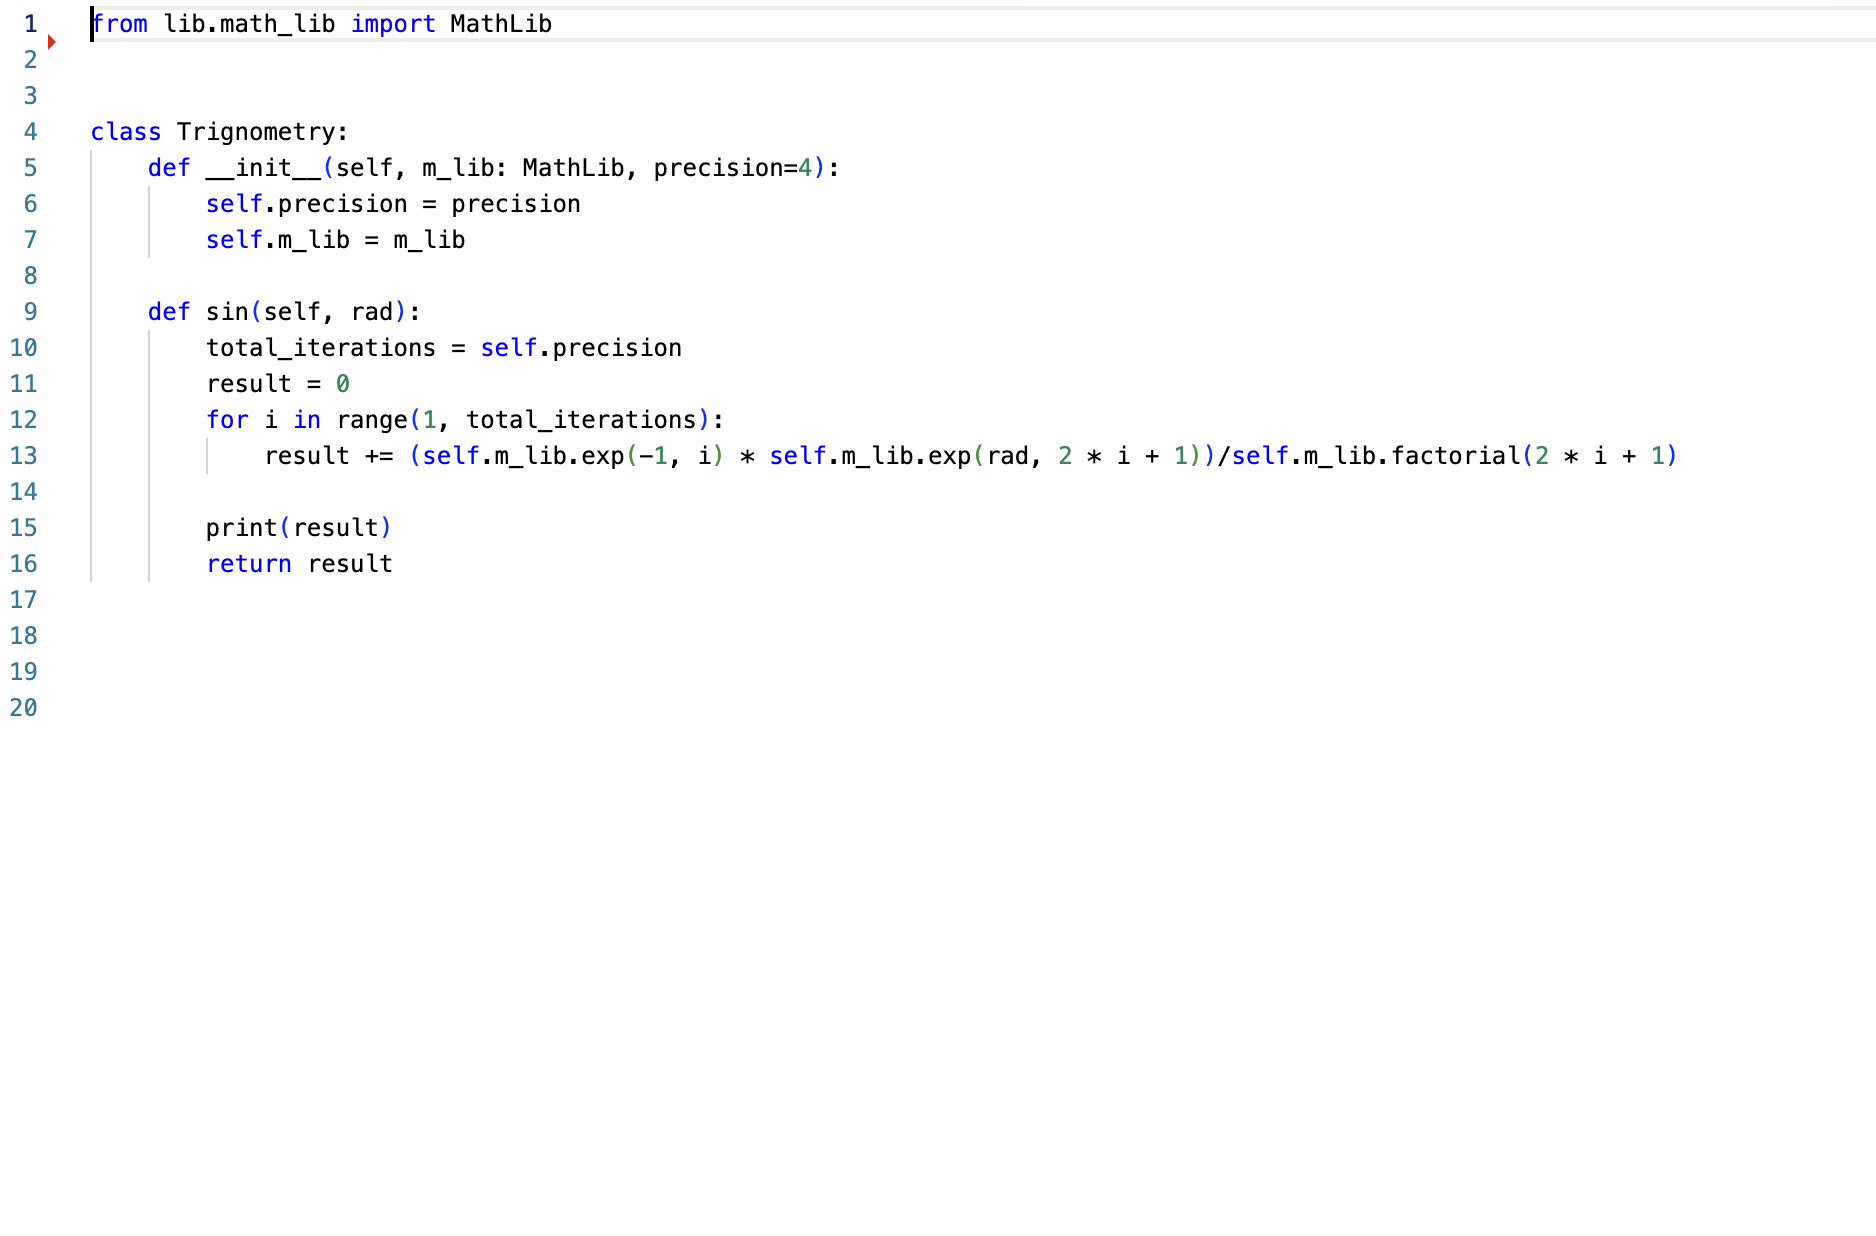
\includegraphics[scale= 0.4]{resources/snippets/Trigonometry.png}}
      \caption{Logic to compute trigonometry functions}
      \label{fig:trigonometric Functions}
    \end{figure}
    \pagebreak

  % \subsection{}
    \begin{itemize}
      \item {The source code was built using the RDD paradigm. This inherently makes it amenable to updates in the future.}
      \item {Adequate comments are provided to make the source code more meaningful to the reader.}
      \item {Since the source code has been broken up into classes and methods, it provides ample opportunities for reuse.}
      \item {Meaningful variables names have been used throughtout the project which makes the code comprehensible.}
      \item {Due to the object-oriented nature of the project design, each class and method in the source code can be unit tested. }
      \item {Each class has it's own set of tests which can verify if the actual output matches the expected.}
      \item {All possible exceptions have been handled throughtout the project and the potential points of failure have been minimized.}
      \item {Any exceptional event which may occur returns meaningful messages to the end user.}
      \item Abstract types have been used to hide the implementation details and improve the composability.
      \item Since the soruce code is (1) Testable and (2) Composable, it in-turn becomes usable. 
    \end{itemize}

    \subsection{Output}
    \begin{figure}[h!]
      \centering
      \frame{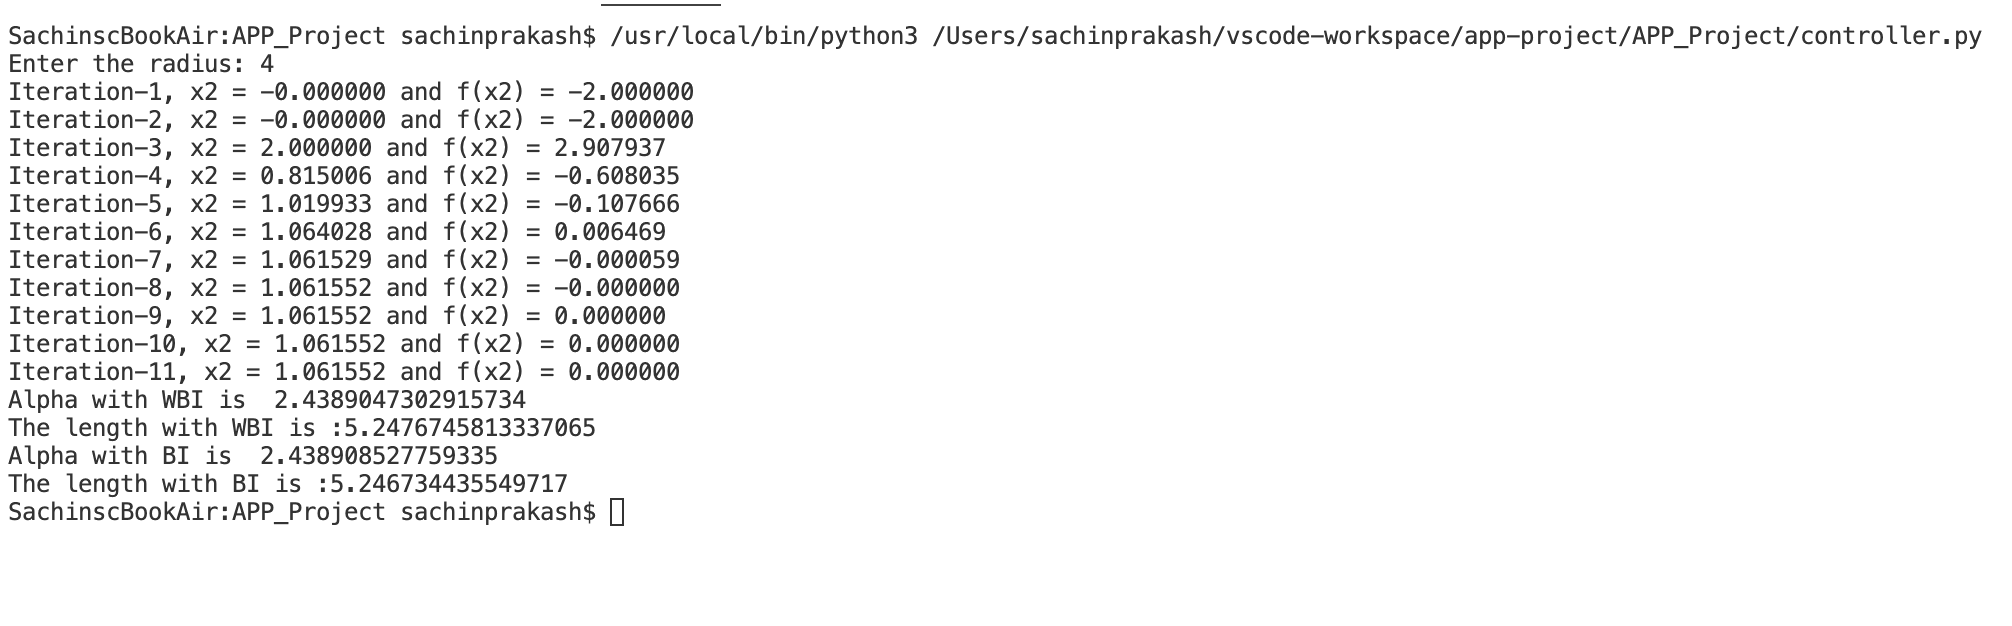
\includegraphics[scale= 0.4]{resources/snippets/inc1OP.png}}
      \caption{Output for Incarnation 1}
      \label{fig:Text-based output}
    \end{figure}
    \pagebreak

% \section{Incarnation 2}]